\documentclass[a4paper,twoside]{article}
\usepackage[T1]{fontenc}
\usepackage[bahasa]{babel}
\usepackage{graphicx}
\usepackage{graphics}
\usepackage{subcaption}
\usepackage{float}
\usepackage[]{hyperref}
\usepackage[cm]{fullpage}
\usepackage{pdflscape} % for landscape full-page images
%\usepackage{multicol} % for multiple columns
\pagestyle{myheadings}
\usepackage{etoolbox}
\usepackage{setspace} 
\usepackage{lipsum} 
\setlength{\headsep}{30pt}
\usepackage[inner=2cm,outer=2.5cm,top=2.5cm,bottom=2cm]{geometry} %margin
% \pagestyle{empty}

\makeatletter
\renewcommand{\@maketitle} {\begin{center} {\LARGE \textbf{ \textsc{\@title}} \par} \bigskip {\large \textbf{\textsc{\@author}} }\end{center} }
\renewcommand{\thispagestyle}[1]{}
\markright{\textbf{\textsc{AIF401/AIF402 \textemdash Rencana Kerja Skripsi \textemdash Sem. Genap 2021/2022}}}

\newcommand{\HRule}{\rule{\linewidth}{0.4mm}}
\renewcommand{\baselinestretch}{1}
\setlength{\parindent}{0 pt}
\setlength{\parskip}{6 pt}

\graphicspath{{./Gambar/}}% folder tempat gambar 
%untuk url dan link
\hypersetup{unicode=true,colorlinks=true,linkcolor=blue,citecolor=green,filecolor=magenta, urlcolor=cyan}

\onehalfspacing

\hyphenation{me-ngu-rangi}

\begin{document}

\title{\@judultopik}
\author{\nama \textendash \@npm} 

%tulis nama dan NPM anda di sini:
\newcommand{\nama}{Alfred Aprianto Liaunardi}
\newcommand{\@npm}{6181801014}
\newcommand{\@judultopik}{Perkakas Command Line KIRI} % Judul/topik anda
\newcommand{\jumpemb}{1} % Jumlah pembimbing, 1 atau 2
\newcommand{\tanggal}{17/03/2022}

% Dokumen hasil template ini harus dicetak bolak-balik !!!!

\maketitle

\pagenumbering{arabic}

\section{Deskripsi}
Semakin pesat perkembangan teknologi, semakin dominan pula penggunaan dan pengaruh teknologi dalam kehidupan kita sehari-hari, salah satunya adalah dalam aspek transportasi. Dengan adanya kendaraan bermotor, seperti mobil dan motor, berpergian ke satu lokasi ke lokasi lainnya berpotensi menjadi lebih mudah, cepat, dan efisien. Seiring dengan perkembangan waktu dan teknologi, sarana transportasi ini menjadi lebih aksesibel ke masyarakat umum, yang menyebabkan semakin banyaknya individu-individu yang memiliki kendaraan bermotor pribadi, dengan beberapa dari mereka bahkan memiliki lebih dari satu.

Dengan bertambahnya kendaraan bermotor yang digunakan oleh masyarakat setiap harinya, timbul \mbox{sebuah} masalah yang sudah membelenggu kota-kota metropolitan selama bertahun-tahun lamanya, yaitu \mbox{kemacetan}. Masalah ini tidak hanya telah menimpa kota-kota besar di seluruh dunia---termasuk di Indonesia, tetapi masalah ini juga tidak menunjukkan tanda-tanda pemulihan selama beberapa tahun terakhir, melainkan dampak-dampak negatif dari kemacetan justru semakin parah, mulai dari pemanasan global, polusi udara, kepadatan tempat parkir kendaraan bermotor, penambahan biaya pemeliharaan infrastruktur bagi pemerintah, penambahan biaya pemeliharaan kendaraan bagi tiap pemiliknya, dan sebagainya.

Oleh karena alasan-alasan di atas, kendaraan umum sebagai alternatif dari kepemilikan kendaraan bermotor pribadi menjadi semakin penting, guna mengurangi kepadatan kendaraan di jalan-jalan raya. Di Indonesia, sudah banyak kendaraan umum yang dikerahkan oleh pemerintah sebagai bentuk dari usaha untuk mengurangi dampak kemacetan ini, salah satunya adalah angkutan kota, atau biasa disingkat sebagai ``angkot'', seperti terlihat pada gambar \ref{fig:angkot}. Sistem yang dimiliki angkot-angkot yang ada sangat sederhana dan mudah dimengerti oleh masyarakat awam sekalipun---tiap angkot memiliki dua buah lokasi yang akan dilewati secara bolak-balik sebagai rute, dan dalam penerapannya pun dapat dikatakan cukup efektif. 

\begin{figure}[H]
	\centering
	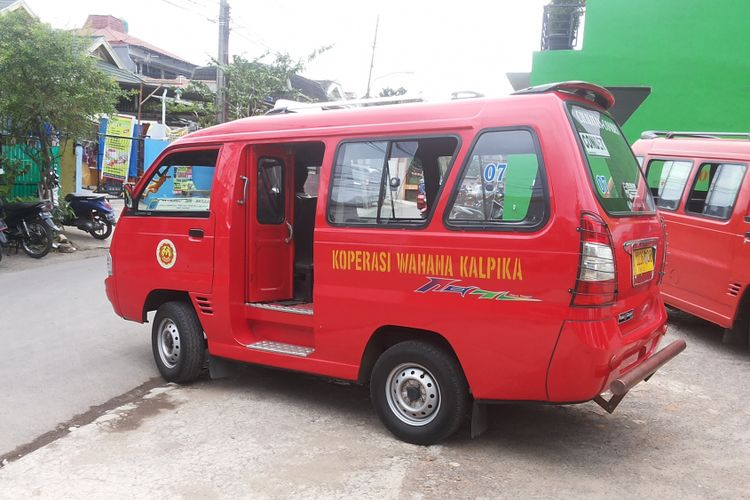
\includegraphics[scale=0.3]{angkot}
	\caption[Angkot yang sedang beroperasi]{Angkutan kota (angkot) yang sedang beroperasi}
	\label{fig:angkot}
\end{figure}

Walaupun begitu, ada salah satu kelemahan fatal dari sistem ini, yaitu kurangnya akses informasi yang dapat dilihat terlebih dahulu oleh penumpang angkot sebelum menggunakan layanan tersebut. Sistem angkot yang ada bergantung pada petunjuk rute---biasanya berupa kode angka atau huruf yang ditempelkan oleh supir angkot pada sisi angkot mereka, Masing-masing kode rute yang berbeda menandakan bahwa angkot tersebut akan menempuh rute yang berbeda. 

% orphan
\vspace*{\fill} \newpage

\begin{figure}[h]
     \centering
     \begin{subfigure}[b]{0.4\textwidth}
         \centering
         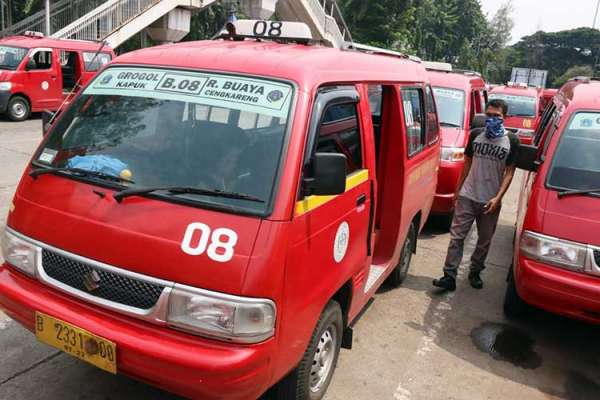
\includegraphics[height=4cm]{angkot-lokasi}
         \caption{Angkot dengan lokasi dan kode rute}
         \vspace{0.5cm}
         \label{fig:angkot-lokasi}
     \end{subfigure}
     \hfill
     \begin{subfigure}[b]{0.5\textwidth}
         \centering
         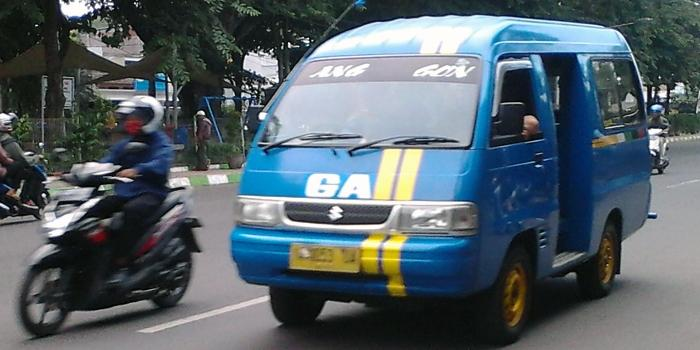
\includegraphics[height=4cm]{angkot-kode}
         \caption{Angkot dengan hanya kode rute}
         \vspace{0.5cm}
         \label{fig:angkot-kode}
     \end{subfigure}
     \begin{subfigure}[b]{\textwidth}
         \centering
         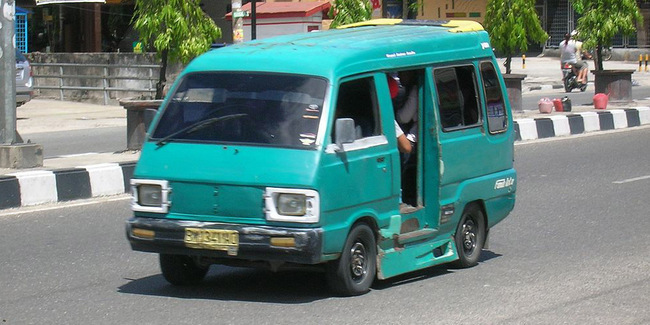
\includegraphics[height=4cm]{angkot-tanpakode}
         \caption{Angkot tanpa lokasi maupun kode rute}
         %\vspace{0.5cm}
         \label{fig:angkot-tanpakode}
     \end{subfigure}
     \caption[Kelengkapan angkot-angkot yang beredar di Indonesia]{Macam-macam kelengkapan kode rute angkot-angkot yang beredar di Indonesia.}
\end{figure}

Hal ini menjadi sebuah kekurangan akibat dua hal utama. Hal pertama adalah bahwa sampai sekarang pun tidak ada akses informasi yang konsisten untuk jalur mana saja yang ditempuh angkot-angkot dengan kode rute tertentu. Sistem yang sangat mengandalkan kode rute ini juga mengandalkan para penumpangnya untuk hafal lokasi mana saja yang dilewati oleh kode rute tertentu, yang sangat sulit untuk dilakukan secara mandiri, akibat tidak adanya panduan yang dapat dilihat mengenai rute mana yang dilewati oleh kode-kode angka tersebut.

Hal kedua adalah bahwa penempelan petunjuk rute di sisi angkot pun seringkali tidak konsisten. Untuk sebagian kecil kasus, terutama di kota-kota besar, beberapa angkot tidak hanya memiliki kode rute, tetapi juga tempelan stiker yang memiliki kedua lokasi yang dilewati dalam rute angkot tersebut, seperi pada gambar \ref{fig:angkot-lokasi}. Sebagian besar dari angkot yang beredaran seringkali hanya memiliki kode rute, seperti terlihat di gambar \ref{fig:angkot-kode}, sedangkan untuk sebagian kasus lainnya, angkot bahkan tidak memiliki petunjuk sama sekali, seperti angkot dalam \ref{fig:angkot-tanpakode}, di mana angkot yang ditunjukkan pada gambar tersebut tidak memiliki stiker lokasi maupun kode rute baik di kaca depan, samping, ataupun belakang.

Permasalahan inilah yang merupakan tujuan dari pencetusan Project KIRI. Project KIRI (atau KIRI saja) adalah sebuah perangkat lunak berbasis web yang dapat menunjukkan rute angkot dari satu titik ke titik lain, mulai dari seberapa jauh pengguna harus berjalan untuk menaiki angkot yang bersangkutan, di mana pengguna harus naik atau turun, seberapa jauh lagi pengguna harus berjalan sampai ke titik tujuan, dan seberapa lama estimasi waktu perjalanan yang akan ditempuh. Tampilan dari halaman web ini dapat dilihat di gambar \ref{fig:kiripage}.

Pada skripsi ini akan dibuat sebuah perangkat lunak berupa perkakas \textit{command line} (\textit{command line tool}) yang dapat menjalankan fungsi-fungsi API dari Project KIRI. Perangkat lunak ini, seperti jenisnya, akan dibuat murni sebagai perkakas yang dijalankan dari \textit{command line} (terminal, cmd, PowerShell, dll.), dan tampilan akhir dari perangkat lunak akan berupa \textit{command line interface} (CLI) tanpa tambahan \textit{graphical user interface} (GUI). Keseluruhan dari perangkat lunak ini akan dibangun dalam bahasa C.

\begin{landscape}
    \begin{figure}[ht]
	    \centering
	    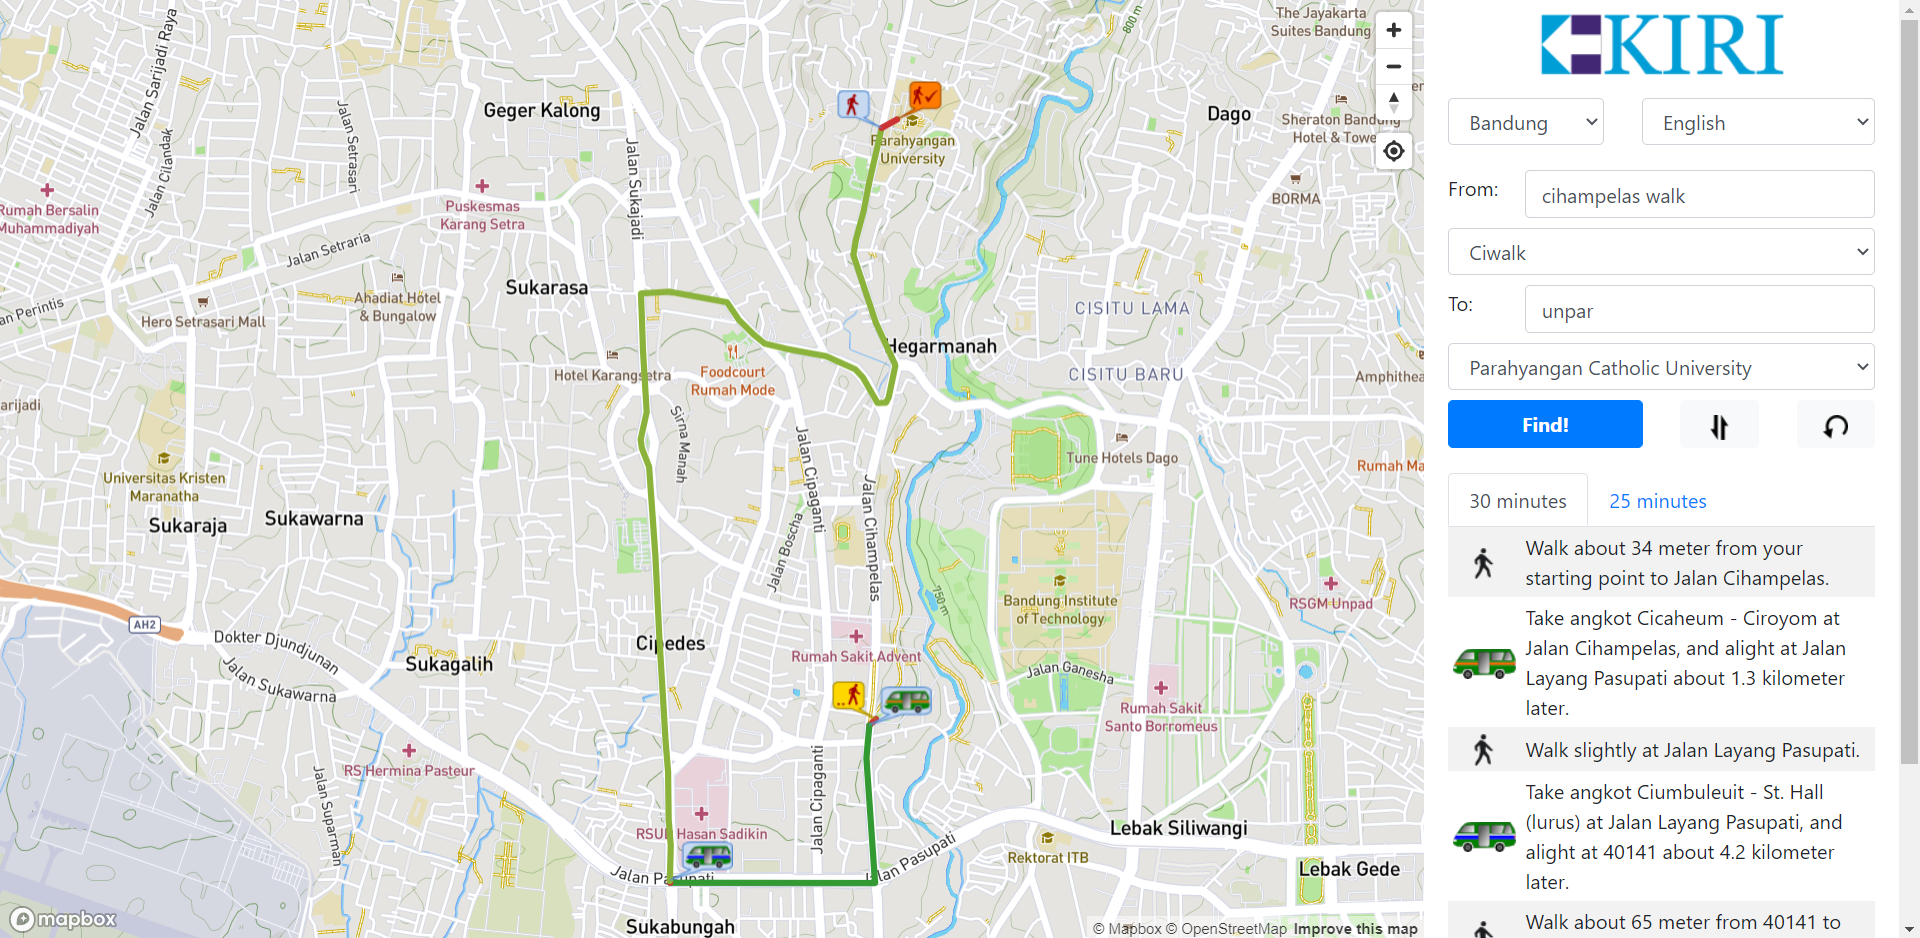
\includegraphics[width=\linewidth]{projectkiri}
	    \caption[Tampilan halaman web Project KIRI]{Tampilan halaman web     \href{https://projectkiri.id}{Project KIRI}, yang menunjukkan rute dari Cihampelas Walk ke Universitas Katolik Parahyangan.}
        \label{fig:kiripage}
    \end{figure}
\end{landscape}

\section{Rumusan Masalah}
\begin{itemize}
	\item Sejauh mana KIRI dapat membantu penumpang angkot untuk mengetahui angkot-angkot mana yang harus dinaiki untuk mencapai lokasi tertentu?
	\item Bagaimana membangun perkakas \textit{command line} yang dapat mengimplementasikan fitur-fitur API KIRI dalam bahasa C?
\end{itemize}

\section{Tujuan}
\begin{itemize}
	\item Mengetahui sejauh mana KIRI dapat membantu penumpang angkot untuk mengetahui angkot-angkot mana yang harus dinaiki untuk mencapai lokasi tertentu.
	\item Membangun perkakas \textit{command line} yang dapat mengimplementasikan fitur-fitur API KIRI dalam bahasa C.
\end{itemize}

\section{Deskripsi Perangkat Lunak}
Perangkat lunak akhir yang akan dibuat memiliki fitur minimal sebagai berikut:
\begin{itemize}
	\item Pengguna dapat memasukkan lokasi awal dan tujuan akhir sebagai masukan dari perangkat lunak.
	\item Pengguna dapat melihat langkah-langkah yang harus ditempuh dalam perjalanan, mulai dari kode-kode angkot mana saja yang harus dinaiki, ke mana pengguna harus berjalan kaki untuk bisa mencapai angkot terdekat dari lokasi terakhir pengguna, sampai seberapa jauh pengguna harus berjalan untuk mencapai tujuan akhir.
	\item Pengguna dapat melihat jarak yang harus ditempuh untuk setiap langkahnya.
	\item Pengguna dapat melihat seberapa lama waktu perjalanan untuk setiap langkahnya.
\end{itemize}

\section{Detail Pengerjaan Skripsi}
Bagian-bagian pekerjaan skripsi ini adalah sebagai berikut :
	\begin{enumerate}
		\item Melakukan eksplorasi fungsi-fungsi perangkat lunak Project KIRI serta explorasi cara implementasi API KIRI.
		\item Mempelajari bahasa pemrograman C serta mempelajari dokumentasi-dokumentasi dari seluruh modul yang dibutuhkan untuk pembuatan perangkat lunak.
		\item Melakukan analisis dan desain perangkat lunak yang akan dibangun.
	    \item Melakukan explorasi terhadap \textit{library-library} yang dapat digunakan serta memenuhi spesifikasi dalam pembuatan perangkat lunak.
		\item Melakukan analisis kebutuhan fitur-fitur perangkat lunak dan melakukan explorasi \textit{library} yang dapat digunakan dan memenuhi spesifikasi dalam pembuatan perangkat lunak.
		\item Membangun perangkat lunak berdasarkan rancangan yang sudah dibuat, dengan megimplementasikan seluruh modul dan \textit{library} yang telah ditentukan di tahap sebelumnya dalam bahasa C.
		\item Melakukan pengujian fungsional dan perbaikan bug (jika ada).
		\item Menulis dokumentasi perangkat lunak.
		\item Menulis dokumen skripsi.
	\end{enumerate}

\section{Rencana Kerja}
Rincian capaian yang direncanakan di Skripsi 1 adalah sebagai berikut:
\begin{enumerate}
    \item Melakukan eksplorasi fungsi-fungsi perangkat lunak Project KIRI serta explorasi cara implementasi API KIRI.
	\item Mempelajari bahasa pemrograman C serta mempelajari dokumentasi-dokumentasi dari seluruh modul yang dibutuhkan untuk pembuatan perangkat lunak.
	\item Melakukan analisis dan desain perangkat lunak yang akan dibangun.
	\item Melakukan explorasi terhadap \textit{library-library} yang dapat digunakan serta memenuhi spesifikasi dalam pembuatan perangkat lunak.
	\item Menulis dokumen skripsi untuk bagian-bagian yang tidak membutuhkan perangkat lunak yang dibuat untuk selesai terlebih dahulu.
\end{enumerate}

Sedangkan yang akan diselesaikan di Skripsi 2 adalah sebagai berikut:
\begin{enumerate}
    \item Membangun perangkat lunak berdasarkan rancangan yang sudah dibuat, dengan megimplementasikan seluruh modul dan \textit{library} yang telah ditentukan di tahap sebelumnya dalam bahasa C.
	\item Melakukan pengujian fungsional dan perbaikan bug (jika ada).
	\item Menulis dokumentasi perangkat lunak.
	\item Menyelesaikan dokumen skripsi.
\end{enumerate}

\vspace{1cm}
\centering Bandung, \tanggal\\
\vspace{2cm} \nama \\ 
\vspace{1cm}

Menyetujui, \\
\ifdefstring{\jumpemb}{2}{
\vspace{1.5cm}
\begin{centering} Menyetujui,\\ \end{centering} \vspace{0.75cm}
\begin{minipage}[b]{0.45\linewidth}
% \centering Bandung, \makebox[0.5cm]{\hrulefill}/\makebox[0.5cm]{\hrulefill}/2013 \\
\vspace{2cm} Nama: \makebox[3cm]{\hrulefill}\\ Pembimbing Utama
\end{minipage} \hspace{0.5cm}
\begin{minipage}[b]{0.45\linewidth}
% \centering Bandung, \makebox[0.5cm]{\hrulefill}/\makebox[0.5cm]{\hrulefill}/2013\\
\vspace{2cm} Nama: \makebox[3cm]{\hrulefill}\\ Pembimbing Pendamping
\end{minipage}
\vspace{0.5cm}
}{
% \centering Bandung, \makebox[0.5cm]{\hrulefill}/\makebox[0.5cm]{\hrulefill}/2013\\
\vspace{2cm} Nama: \makebox[3cm]{\hrulefill}\\ Pembimbing Tunggal
}

\end{document}